\documentclass[twoside]{article}
\usepackage{graphicx}
\usepackage{listings}
\usepackage{xcolor}
\usepackage{tabularx}
\usepackage{amsmath}
\usepackage{hyperref}
\usepackage{tikz}
\usepackage{blindtext}
\usepackage{titlesec}
\usepackage{pgfplots}
\usepackage{fancyhdr}
\usepackage{hyperref}
\usepackage{array}

\definecolor{codegreen}{rgb}{0,0.6,0}
\definecolor{codegray}{rgb}{0.5,0.5,0.5}
\definecolor{codepurple}{rgb}{0.58,0,0.82}
\definecolor{backcolour}{rgb}{0.95,0.95,0.92}

\lstdefinestyle{mystyle}{
    backgroundcolor=\color{backcolour},   
    commentstyle=\color{codegreen},
    keywordstyle=\color{magenta},
    numberstyle=\tiny\color{codegray},
    stringstyle=\color{codepurple},
    basicstyle=\ttfamily\footnotesize,
    breakatwhitespace=false,         
    breaklines=true,                 
    captionpos=b,                    
    keepspaces=true,                 
    % numbers=left,                    
    % numbersep=5pt,                  
    showspaces=false,                
    showstringspaces=false,
    showtabs=true,                  
    tabsize=4
}

\lstset{style=mystyle}

\title{Hand-written Digit Recognition using Numpy}
\author{Yashwant Bhosale}
\date{January 2025}

\pagestyle{fancy}
%... then configure it.
\fancyhead{} % clear all header fields
\fancyhead[RO,LE]{\textbf{Handwritten Digit Recognition using NumPy}}

\begin{document}
\maketitle

\hypersetup{pdfborder= 0 0 0}
\tableofcontents
\newpage

\section{Overview}
This project demonstrates working of a simple neural network using the MNIST dataset. The special thing about this project is that it is implemented only using \underline{numpy} and no other libraries. The neural network is trained using the \textit{backpropagation algorithm}. The neural network is trained on the MNIST dataset and is able to achieve an accuracy of 97.8\% on the test dataset. The project also contains a simple web interface to draw digits and predict the digit using the trained neural network.

\subsection{Dataset}
The neural network is trained on \textbf{MNIST Dataset}. It is set of about 70,000 images divided into training data and testing data. Training data contains 60,000 images and testing data contains 10,000 images.

\subsection{Technologies used}
The approach of this project was to learn how neural networks work by implementing them from scratch.
So, the neural network is written in python and only using NumPy which is popular library in python used to deal with numbers.

\subsection{Approach}
The appoach is layered-neural network. The neural network has
\begin{enumerate}
    \item \textbf{Input layer:} It has 784 neurons. Each image in dataset is 28 pixels wide and 28 pixels long. This layer is constructed by flattening array of RGBA values of pixels of a 28x28 image.
    \item \textbf{Hidden layers:} My network contains two hidden layers one having 128 neurons and other having 64 neurons. These layers play important role of capturing features of each image.
    \item \textbf{Output layer:} Output layer contains 10 neurons representing 10 digits. Network will try to confidently classify image as one of the 10 digits.
\end{enumerate}

\section{Parts of Neural Network}
\begin{figure}
    \centering
    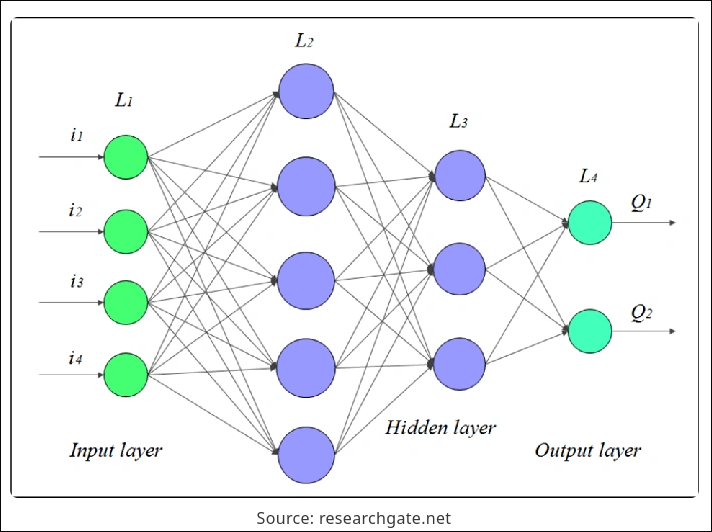
\includegraphics[scale=0.3]{image.png}
    \caption{Example image demonstrating neural networks}
    \label{fig:enter-label}
\end{figure}


There are various elements that constitute a neural network. It is essential to know what is significance of each of them:

\begin{itemize}
    \item \textbf{Neuron}: Neuron can be looked at as a simple container that holds some value. There are layers in the network and each layer contains some neurons. Activation of neurons in one layer defines the activations in the next and so on.
    \item \textbf{layers}: There are layers in the neural network and it can be seen in the image.
    You may look at layers as something which is expected to record some specific feature of the image. 
    \item \textbf{Weights and Biases}: Weights and biases are parameters in neural networks that control the strength of connections between neurons and the output of the network. They are learned during the training process and are adjusted to optimize the network's performance
    \item \textbf{Cost function}: A cost function in a neural network is a measure of how far the predicted output is from the actual output. It's also known as a loss function. We essentially look at how wrong are we.
    \item \textbf{Activation function}: An activation function is a mathematical function applied to the output of a neuron. It introduces non-linearity into the model, allowing the network to learn and represent complex patterns in the data. 
\end{itemize}

\[ a^L = w^{L-1} \cdot a^{L-1} + b^{L-1} \]
\\
\(a^L\): Neuron activations in \(L^{th}\) layer\\
\(w^{L-1}\): weights of \((L-1)^{th}\) layer\\
\(a^{L-1}\): Neuron activations in \((L-1)^{th}\) layer\\
\(b^{L-1}\): Biases of  \((L-1)^{th}\) layer\\
\\
This function sort of \textbf{governs} the neural networks. You may understand this as we discussed earlier activations, weights and biases of one layer determine the activation in the next layer.
\\
Examples of cost functions:
\begin{itemize}
    \item \textbf{Mean Square Error}: 
    \[Cost = \sum_{i=1}^{n} (y - y_i)^2\]
    \item \textbf{Cross Entropy Loss}
    \[Cost = -{(y\log(p) + (1 - y)\log(1 - p))}\]
\end{itemize}



\section{Technical concepts}

This section demonstrates the usage of advanced LaTeX features including equations, hyperlinks, tables, lists, and diagrams.

\subsection{Mathematical Equations}
Here is an example of a mathematical equation used for weight updates in backpropagation:
\begin{align}
    w_{ij}^{(t+1)} &= w_{ij}^{(t)} - \eta \frac{\partial C}{\partial w_{ij}} \\
    b_j^{(t+1)} &= b_j^{(t)} - \eta \frac{\partial C}{\partial b_j},
\end{align}
where:
\begin{itemize}
    \item \( w_{ij} \): Weight between neuron \(i\) in layer \(L\) and neuron \(j\) in layer \(L+1\)
    \item \( \eta \): Learning rate
    \item \( \frac{\partial C}{\partial w_{ij}} \): Gradient of cost function
\end{itemize}

\subsection{Dataset}
For more information on the MNIST dataset, visit the official \href{https://www.kaggle.com/datasets/hojjatk/mnist-dataset}{MNIST Database website}.

\subsection{Different activation function}
The following table illustrates a comparison of activation functions:
\begin{center}
\vspace{1cm}
u8i\begin{tabular}{|c|c|c|}
\hline
\textbf{Activation Function} & \textbf{Formula} & \textbf{Range} \\[5px]
\hline
Sigmoid & \( \sigma(x) = \frac{1}{1 + e^{-x}} \) & (0, 1) \\[5px]
\hline
ReLU & \( f(x) = \max(0, x) \) & [0, \( \infty \)] \\[5px]
\hline
Tanh & \( f(x) = \frac{e^x - e^{-x}}{e^x + e^{-x}} \) & (-1, 1) \\[5px]
\hline
\end{tabular}
\end{center}

\subsection{High level diagram}
Below is a simple diagram describing neural network
\begin{center}
% \usetikzlibrary {arrows.meta} 
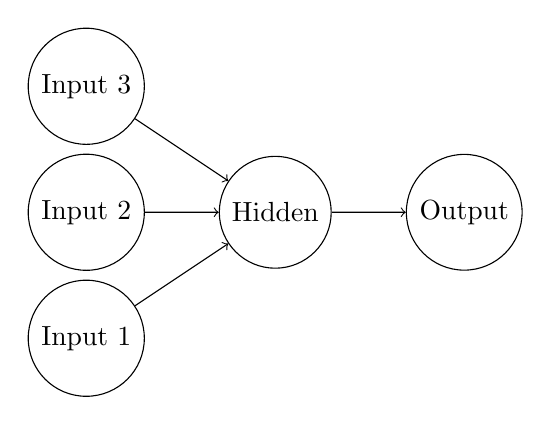
\begin{tikzpicture}[scale=0.8, every node/.style={circle, draw}]
  \node (n1) at (0, 0) {Input 1};
  \node (n2) at (0, 2) {Input 2};
  \node (n3) at (0, 4) {Input 3};
  \node (h1) at (3, 2) {Hidden};
  \node (o) at (6, 2) {Output};

  \draw[->] (n1) -- (h1);
  \draw[->] (n2) -- (h1);
  \draw[->] (n3) -- (h1);
  \draw[->] (h1) -- (o);
\end{tikzpicture}
\end{center}

\subsection{Code Blocks}
The following is an example Python code snippet demonstrating weight initialization:
\begin{lstlisting}[language=Python, caption=Weight Initialization]
import numpy as np
weights = np.random.randn(784, 128) * 0.01
biases = np.zeros((128, 1))
\end{lstlisting}

\subsection{How to train a neural network}
Steps for training a neural network:
\begin{enumerate}
    \item Initialize weights and biases.
    \item Feedforward to compute outputs.
    \item Compute the cost function.
    \item Backpropagate to update weights.
    \item Repeat until convergence.
\end{enumerate}

\section {Testing}
\begin{tikzpicture}
  \begin{axis} [axis lines=center]
    \addplot [domain=-3:3, smooth, thick] { sin(deg(x)) };
  \end{axis}
\end{tikzpicture}
\\
\\
The equation of straight line in intercept form is \( y = mx + c \)


\section*{Data Table with Links}

Here is a table where each row links to multiple external files.

\begin{table}[h]
    \centering
    \begin{tabular}{|c|c|c|}
        \hline
        Data Name & File 1 & File 2 \\
        \hline
        Experiment A & \href{run:expA_data1.pdf}{Data 1} & \href{run:expA_data2.csv}{Data 2} \\
        \hline
        Experiment B & \href{file:///home/yashwantbhosale/Downloads/Ch%202-1.pdf}{Report} & \href{run:expB_data2.txt}{Raw Data} \\
        \hline
        Experiment C & \href{https://www.tensorflow.org/datasets/catalog/mnist}{Dataset C} & \href{run:expC_notes.pdf}{Notes} \\
        \hline
    \end{tabular}
    \caption{Table with links to multiple external files}
    \label{tab:data_links}
\end{table}

\end{document}


